\begin{figure}[H]
  \centering
  \begin{subfigure}[t]{.48\linewidth}
    \centering
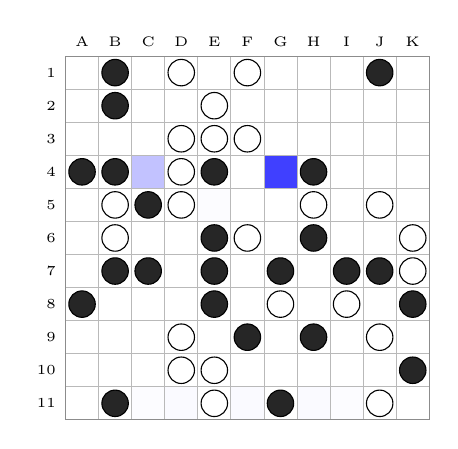
\begin{tikzpicture}[x=0.42cm, y=0.42cm]
\fill[blue!24] (2,-3) rectangle (3,-4);
\fill[blue!75] (6,-3) rectangle (7,-4);
\fill[blue!1] (4,-4) rectangle (5,-5);
\fill[blue!1] (2,-10) rectangle (3,-11);
\fill[blue!2] (3,-10) rectangle (4,-11);
\fill[blue!2] (5,-10) rectangle (6,-11);
\fill[blue!2] (7,-10) rectangle (8,-11);
\fill[blue!1] (8,-10) rectangle (9,-11);
\draw[gray!55, line width=.3pt, step=1] (0,0) grid (11,-11);
\draw[gray!90] (0,0) rectangle (11,-11);
\node[font=\tiny, anchor=south] at (0.5,0) {A};
\node[font=\tiny, anchor=south] at (1.5,0) {B};
\node[font=\tiny, anchor=south] at (2.5,0) {C};
\node[font=\tiny, anchor=south] at (3.5,0) {D};
\node[font=\tiny, anchor=south] at (4.5,0) {E};
\node[font=\tiny, anchor=south] at (5.5,0) {F};
\node[font=\tiny, anchor=south] at (6.5,0) {G};
\node[font=\tiny, anchor=south] at (7.5,0) {H};
\node[font=\tiny, anchor=south] at (8.5,0) {I};
\node[font=\tiny, anchor=south] at (9.5,0) {J};
\node[font=\tiny, anchor=south] at (10.5,0) {K};
\node[font=\tiny, anchor=east] at (0,-0.5) {1};
\node[font=\tiny, anchor=east] at (0,-1.5) {2};
\node[font=\tiny, anchor=east] at (0,-2.5) {3};
\node[font=\tiny, anchor=east] at (0,-3.5) {4};
\node[font=\tiny, anchor=east] at (0,-4.5) {5};
\node[font=\tiny, anchor=east] at (0,-5.5) {6};
\node[font=\tiny, anchor=east] at (0,-6.5) {7};
\node[font=\tiny, anchor=east] at (0,-7.5) {8};
\node[font=\tiny, anchor=east] at (0,-8.5) {9};
\node[font=\tiny, anchor=east] at (0,-9.5) {10};
\node[font=\tiny, anchor=east] at (0,-10.5) {11};
\draw[fill=black!85, line width=.4pt] (1.5,-0.5) circle (.40);
\draw[fill=white, line width=.4pt] (3.5,-0.5) circle (.40);
\draw[fill=white, line width=.4pt] (5.5,-0.5) circle (.40);
\draw[fill=black!85, line width=.4pt] (9.5,-0.5) circle (.40);
\draw[fill=black!85, line width=.4pt] (1.5,-1.5) circle (.40);
\draw[fill=white, line width=.4pt] (4.5,-1.5) circle (.40);
\draw[fill=white, line width=.4pt] (3.5,-2.5) circle (.40);
\draw[fill=white, line width=.4pt] (4.5,-2.5) circle (.40);
\draw[fill=white, line width=.4pt] (5.5,-2.5) circle (.40);
\draw[fill=black!85, line width=.4pt] (0.5,-3.5) circle (.40);
\draw[fill=black!85, line width=.4pt] (1.5,-3.5) circle (.40);
\draw[fill=white, line width=.4pt] (3.5,-3.5) circle (.40);
\draw[fill=black!85, line width=.4pt] (4.5,-3.5) circle (.40);
\draw[fill=black!85, line width=.4pt] (7.5,-3.5) circle (.40);
\draw[fill=white, line width=.4pt] (1.5,-4.5) circle (.40);
\draw[fill=black!85, line width=.4pt] (2.5,-4.5) circle (.40);
\draw[fill=white, line width=.4pt] (3.5,-4.5) circle (.40);
\draw[fill=white, line width=.4pt] (7.5,-4.5) circle (.40);
\draw[fill=white, line width=.4pt] (9.5,-4.5) circle (.40);
\draw[fill=white, line width=.4pt] (1.5,-5.5) circle (.40);
\draw[fill=black!85, line width=.4pt] (4.5,-5.5) circle (.40);
\draw[fill=white, line width=.4pt] (5.5,-5.5) circle (.40);
\draw[fill=black!85, line width=.4pt] (7.5,-5.5) circle (.40);
\draw[fill=white, line width=.4pt] (10.5,-5.5) circle (.40);
\draw[fill=black!85, line width=.4pt] (1.5,-6.5) circle (.40);
\draw[fill=black!85, line width=.4pt] (2.5,-6.5) circle (.40);
\draw[fill=black!85, line width=.4pt] (4.5,-6.5) circle (.40);
\draw[fill=black!85, line width=.4pt] (6.5,-6.5) circle (.40);
\draw[fill=black!85, line width=.4pt] (8.5,-6.5) circle (.40);
\draw[fill=black!85, line width=.4pt] (9.5,-6.5) circle (.40);
\draw[fill=white, line width=.4pt] (10.5,-6.5) circle (.40);
\draw[fill=black!85, line width=.4pt] (0.5,-7.5) circle (.40);
\draw[fill=black!85, line width=.4pt] (4.5,-7.5) circle (.40);
\draw[fill=white, line width=.4pt] (6.5,-7.5) circle (.40);
\draw[fill=white, line width=.4pt] (8.5,-7.5) circle (.40);
\draw[fill=black!85, line width=.4pt] (10.5,-7.5) circle (.40);
\draw[fill=white, line width=.4pt] (3.5,-8.5) circle (.40);
\draw[fill=black!85, line width=.4pt] (5.5,-8.5) circle (.40);
\draw[fill=black!85, line width=.4pt] (7.5,-8.5) circle (.40);
\draw[fill=white, line width=.4pt] (9.5,-8.5) circle (.40);
\draw[fill=white, line width=.4pt] (3.5,-9.5) circle (.40);
\draw[fill=white, line width=.4pt] (4.5,-9.5) circle (.40);
\draw[fill=black!85, line width=.4pt] (10.5,-9.5) circle (.40);
\draw[fill=black!85, line width=.4pt] (1.5,-10.5) circle (.40);
\draw[fill=white, line width=.4pt] (4.5,-10.5) circle (.40);
\draw[fill=black!85, line width=.4pt] (6.5,-10.5) circle (.40);
\draw[fill=white, line width=.4pt] (9.5,-10.5) circle (.40);
\end{tikzpicture}
    \caption{SL v3: $v=0{,}87$; đáp án 90,0\%; cao nhất G4 (68,1\%)}
  \end{subfigure}\hfill
  \begin{subfigure}[t]{.48\linewidth}
    \centering
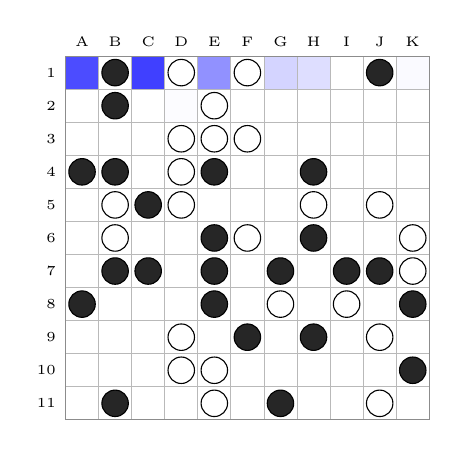
\begin{tikzpicture}[x=0.42cm, y=0.42cm]
\fill[blue!70] (0,0) rectangle (1,-1);
\fill[blue!75] (2,0) rectangle (3,-1);
\fill[blue!43] (4,0) rectangle (5,-1);
\fill[blue!17] (6,0) rectangle (7,-1);
\fill[blue!13] (7,0) rectangle (8,-1);
\fill[blue!2] (10,0) rectangle (11,-1);
\fill[blue!1] (3,-1) rectangle (4,-2);
\draw[gray!55, line width=.3pt, step=1] (0,0) grid (11,-11);
\draw[gray!90] (0,0) rectangle (11,-11);
\node[font=\tiny, anchor=south] at (0.5,0) {A};
\node[font=\tiny, anchor=south] at (1.5,0) {B};
\node[font=\tiny, anchor=south] at (2.5,0) {C};
\node[font=\tiny, anchor=south] at (3.5,0) {D};
\node[font=\tiny, anchor=south] at (4.5,0) {E};
\node[font=\tiny, anchor=south] at (5.5,0) {F};
\node[font=\tiny, anchor=south] at (6.5,0) {G};
\node[font=\tiny, anchor=south] at (7.5,0) {H};
\node[font=\tiny, anchor=south] at (8.5,0) {I};
\node[font=\tiny, anchor=south] at (9.5,0) {J};
\node[font=\tiny, anchor=south] at (10.5,0) {K};
\node[font=\tiny, anchor=east] at (0,-0.5) {1};
\node[font=\tiny, anchor=east] at (0,-1.5) {2};
\node[font=\tiny, anchor=east] at (0,-2.5) {3};
\node[font=\tiny, anchor=east] at (0,-3.5) {4};
\node[font=\tiny, anchor=east] at (0,-4.5) {5};
\node[font=\tiny, anchor=east] at (0,-5.5) {6};
\node[font=\tiny, anchor=east] at (0,-6.5) {7};
\node[font=\tiny, anchor=east] at (0,-7.5) {8};
\node[font=\tiny, anchor=east] at (0,-8.5) {9};
\node[font=\tiny, anchor=east] at (0,-9.5) {10};
\node[font=\tiny, anchor=east] at (0,-10.5) {11};
\draw[fill=black!85, line width=.4pt] (1.5,-0.5) circle (.40);
\draw[fill=white, line width=.4pt] (3.5,-0.5) circle (.40);
\draw[fill=white, line width=.4pt] (5.5,-0.5) circle (.40);
\draw[fill=black!85, line width=.4pt] (9.5,-0.5) circle (.40);
\draw[fill=black!85, line width=.4pt] (1.5,-1.5) circle (.40);
\draw[fill=white, line width=.4pt] (4.5,-1.5) circle (.40);
\draw[fill=white, line width=.4pt] (3.5,-2.5) circle (.40);
\draw[fill=white, line width=.4pt] (4.5,-2.5) circle (.40);
\draw[fill=white, line width=.4pt] (5.5,-2.5) circle (.40);
\draw[fill=black!85, line width=.4pt] (0.5,-3.5) circle (.40);
\draw[fill=black!85, line width=.4pt] (1.5,-3.5) circle (.40);
\draw[fill=white, line width=.4pt] (3.5,-3.5) circle (.40);
\draw[fill=black!85, line width=.4pt] (4.5,-3.5) circle (.40);
\draw[fill=black!85, line width=.4pt] (7.5,-3.5) circle (.40);
\draw[fill=white, line width=.4pt] (1.5,-4.5) circle (.40);
\draw[fill=black!85, line width=.4pt] (2.5,-4.5) circle (.40);
\draw[fill=white, line width=.4pt] (3.5,-4.5) circle (.40);
\draw[fill=white, line width=.4pt] (7.5,-4.5) circle (.40);
\draw[fill=white, line width=.4pt] (9.5,-4.5) circle (.40);
\draw[fill=white, line width=.4pt] (1.5,-5.5) circle (.40);
\draw[fill=black!85, line width=.4pt] (4.5,-5.5) circle (.40);
\draw[fill=white, line width=.4pt] (5.5,-5.5) circle (.40);
\draw[fill=black!85, line width=.4pt] (7.5,-5.5) circle (.40);
\draw[fill=white, line width=.4pt] (10.5,-5.5) circle (.40);
\draw[fill=black!85, line width=.4pt] (1.5,-6.5) circle (.40);
\draw[fill=black!85, line width=.4pt] (2.5,-6.5) circle (.40);
\draw[fill=black!85, line width=.4pt] (4.5,-6.5) circle (.40);
\draw[fill=black!85, line width=.4pt] (6.5,-6.5) circle (.40);
\draw[fill=black!85, line width=.4pt] (8.5,-6.5) circle (.40);
\draw[fill=black!85, line width=.4pt] (9.5,-6.5) circle (.40);
\draw[fill=white, line width=.4pt] (10.5,-6.5) circle (.40);
\draw[fill=black!85, line width=.4pt] (0.5,-7.5) circle (.40);
\draw[fill=black!85, line width=.4pt] (4.5,-7.5) circle (.40);
\draw[fill=white, line width=.4pt] (6.5,-7.5) circle (.40);
\draw[fill=white, line width=.4pt] (8.5,-7.5) circle (.40);
\draw[fill=black!85, line width=.4pt] (10.5,-7.5) circle (.40);
\draw[fill=white, line width=.4pt] (3.5,-8.5) circle (.40);
\draw[fill=black!85, line width=.4pt] (5.5,-8.5) circle (.40);
\draw[fill=black!85, line width=.4pt] (7.5,-8.5) circle (.40);
\draw[fill=white, line width=.4pt] (9.5,-8.5) circle (.40);
\draw[fill=white, line width=.4pt] (3.5,-9.5) circle (.40);
\draw[fill=white, line width=.4pt] (4.5,-9.5) circle (.40);
\draw[fill=black!85, line width=.4pt] (10.5,-9.5) circle (.40);
\draw[fill=black!85, line width=.4pt] (1.5,-10.5) circle (.40);
\draw[fill=white, line width=.4pt] (4.5,-10.5) circle (.40);
\draw[fill=black!85, line width=.4pt] (6.5,-10.5) circle (.40);
\draw[fill=white, line width=.4pt] (9.5,-10.5) circle (.40);
\end{tikzpicture}
    \caption{SL không aug: $v=0{,}38$; đáp án 1,0\%; cao nhất C1 (33,5\%)}
  \end{subfigure}\par\medskip
  \begin{subfigure}[t]{.48\linewidth}
    \centering
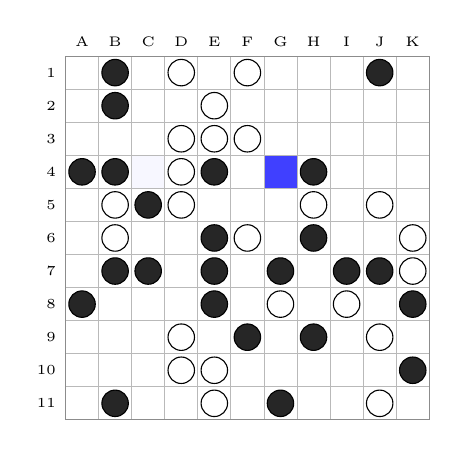
\begin{tikzpicture}[x=0.42cm, y=0.42cm]
\fill[blue!3] (2,-3) rectangle (3,-4);
\fill[blue!75] (6,-3) rectangle (7,-4);
\draw[gray!55, line width=.3pt, step=1] (0,0) grid (11,-11);
\draw[gray!90] (0,0) rectangle (11,-11);
\node[font=\tiny, anchor=south] at (0.5,0) {A};
\node[font=\tiny, anchor=south] at (1.5,0) {B};
\node[font=\tiny, anchor=south] at (2.5,0) {C};
\node[font=\tiny, anchor=south] at (3.5,0) {D};
\node[font=\tiny, anchor=south] at (4.5,0) {E};
\node[font=\tiny, anchor=south] at (5.5,0) {F};
\node[font=\tiny, anchor=south] at (6.5,0) {G};
\node[font=\tiny, anchor=south] at (7.5,0) {H};
\node[font=\tiny, anchor=south] at (8.5,0) {I};
\node[font=\tiny, anchor=south] at (9.5,0) {J};
\node[font=\tiny, anchor=south] at (10.5,0) {K};
\node[font=\tiny, anchor=east] at (0,-0.5) {1};
\node[font=\tiny, anchor=east] at (0,-1.5) {2};
\node[font=\tiny, anchor=east] at (0,-2.5) {3};
\node[font=\tiny, anchor=east] at (0,-3.5) {4};
\node[font=\tiny, anchor=east] at (0,-4.5) {5};
\node[font=\tiny, anchor=east] at (0,-5.5) {6};
\node[font=\tiny, anchor=east] at (0,-6.5) {7};
\node[font=\tiny, anchor=east] at (0,-7.5) {8};
\node[font=\tiny, anchor=east] at (0,-8.5) {9};
\node[font=\tiny, anchor=east] at (0,-9.5) {10};
\node[font=\tiny, anchor=east] at (0,-10.5) {11};
\draw[fill=black!85, line width=.4pt] (1.5,-0.5) circle (.40);
\draw[fill=white, line width=.4pt] (3.5,-0.5) circle (.40);
\draw[fill=white, line width=.4pt] (5.5,-0.5) circle (.40);
\draw[fill=black!85, line width=.4pt] (9.5,-0.5) circle (.40);
\draw[fill=black!85, line width=.4pt] (1.5,-1.5) circle (.40);
\draw[fill=white, line width=.4pt] (4.5,-1.5) circle (.40);
\draw[fill=white, line width=.4pt] (3.5,-2.5) circle (.40);
\draw[fill=white, line width=.4pt] (4.5,-2.5) circle (.40);
\draw[fill=white, line width=.4pt] (5.5,-2.5) circle (.40);
\draw[fill=black!85, line width=.4pt] (0.5,-3.5) circle (.40);
\draw[fill=black!85, line width=.4pt] (1.5,-3.5) circle (.40);
\draw[fill=white, line width=.4pt] (3.5,-3.5) circle (.40);
\draw[fill=black!85, line width=.4pt] (4.5,-3.5) circle (.40);
\draw[fill=black!85, line width=.4pt] (7.5,-3.5) circle (.40);
\draw[fill=white, line width=.4pt] (1.5,-4.5) circle (.40);
\draw[fill=black!85, line width=.4pt] (2.5,-4.5) circle (.40);
\draw[fill=white, line width=.4pt] (3.5,-4.5) circle (.40);
\draw[fill=white, line width=.4pt] (7.5,-4.5) circle (.40);
\draw[fill=white, line width=.4pt] (9.5,-4.5) circle (.40);
\draw[fill=white, line width=.4pt] (1.5,-5.5) circle (.40);
\draw[fill=black!85, line width=.4pt] (4.5,-5.5) circle (.40);
\draw[fill=white, line width=.4pt] (5.5,-5.5) circle (.40);
\draw[fill=black!85, line width=.4pt] (7.5,-5.5) circle (.40);
\draw[fill=white, line width=.4pt] (10.5,-5.5) circle (.40);
\draw[fill=black!85, line width=.4pt] (1.5,-6.5) circle (.40);
\draw[fill=black!85, line width=.4pt] (2.5,-6.5) circle (.40);
\draw[fill=black!85, line width=.4pt] (4.5,-6.5) circle (.40);
\draw[fill=black!85, line width=.4pt] (6.5,-6.5) circle (.40);
\draw[fill=black!85, line width=.4pt] (8.5,-6.5) circle (.40);
\draw[fill=black!85, line width=.4pt] (9.5,-6.5) circle (.40);
\draw[fill=white, line width=.4pt] (10.5,-6.5) circle (.40);
\draw[fill=black!85, line width=.4pt] (0.5,-7.5) circle (.40);
\draw[fill=black!85, line width=.4pt] (4.5,-7.5) circle (.40);
\draw[fill=white, line width=.4pt] (6.5,-7.5) circle (.40);
\draw[fill=white, line width=.4pt] (8.5,-7.5) circle (.40);
\draw[fill=black!85, line width=.4pt] (10.5,-7.5) circle (.40);
\draw[fill=white, line width=.4pt] (3.5,-8.5) circle (.40);
\draw[fill=black!85, line width=.4pt] (5.5,-8.5) circle (.40);
\draw[fill=black!85, line width=.4pt] (7.5,-8.5) circle (.40);
\draw[fill=white, line width=.4pt] (9.5,-8.5) circle (.40);
\draw[fill=white, line width=.4pt] (3.5,-9.5) circle (.40);
\draw[fill=white, line width=.4pt] (4.5,-9.5) circle (.40);
\draw[fill=black!85, line width=.4pt] (10.5,-9.5) circle (.40);
\draw[fill=black!85, line width=.4pt] (1.5,-10.5) circle (.40);
\draw[fill=white, line width=.4pt] (4.5,-10.5) circle (.40);
\draw[fill=black!85, line width=.4pt] (6.5,-10.5) circle (.40);
\draw[fill=white, line width=.4pt] (9.5,-10.5) circle (.40);
\end{tikzpicture}
    \caption{L6 (RL): $v=1{,}00$; đáp án 99,6\%; cao nhất G4 (95,9\%)}
  \end{subfigure}\hfill
  \begin{subfigure}[t]{.48\linewidth}
    \centering
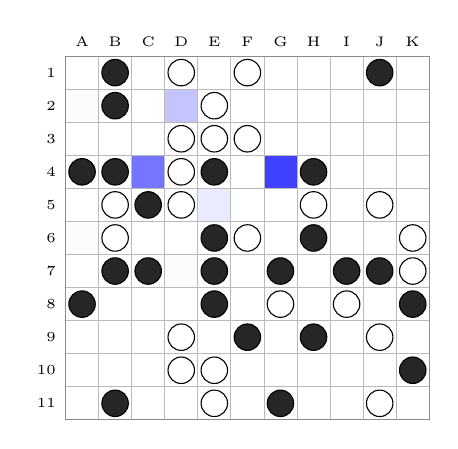
\begin{tikzpicture}[x=0.42cm, y=0.42cm]
\fill[blue!1] (0,-1) rectangle (1,-2);
\fill[blue!23] (3,-1) rectangle (4,-2);
\fill[blue!54] (2,-3) rectangle (3,-4);
\fill[blue!75] (6,-3) rectangle (7,-4);
\fill[blue!8] (4,-4) rectangle (5,-5);
\fill[blue!1] (0,-5) rectangle (1,-6);
\fill[blue!1] (3,-6) rectangle (4,-7);
\draw[gray!55, line width=.3pt, step=1] (0,0) grid (11,-11);
\draw[gray!90] (0,0) rectangle (11,-11);
\node[font=\tiny, anchor=south] at (0.5,0) {A};
\node[font=\tiny, anchor=south] at (1.5,0) {B};
\node[font=\tiny, anchor=south] at (2.5,0) {C};
\node[font=\tiny, anchor=south] at (3.5,0) {D};
\node[font=\tiny, anchor=south] at (4.5,0) {E};
\node[font=\tiny, anchor=south] at (5.5,0) {F};
\node[font=\tiny, anchor=south] at (6.5,0) {G};
\node[font=\tiny, anchor=south] at (7.5,0) {H};
\node[font=\tiny, anchor=south] at (8.5,0) {I};
\node[font=\tiny, anchor=south] at (9.5,0) {J};
\node[font=\tiny, anchor=south] at (10.5,0) {K};
\node[font=\tiny, anchor=east] at (0,-0.5) {1};
\node[font=\tiny, anchor=east] at (0,-1.5) {2};
\node[font=\tiny, anchor=east] at (0,-2.5) {3};
\node[font=\tiny, anchor=east] at (0,-3.5) {4};
\node[font=\tiny, anchor=east] at (0,-4.5) {5};
\node[font=\tiny, anchor=east] at (0,-5.5) {6};
\node[font=\tiny, anchor=east] at (0,-6.5) {7};
\node[font=\tiny, anchor=east] at (0,-7.5) {8};
\node[font=\tiny, anchor=east] at (0,-8.5) {9};
\node[font=\tiny, anchor=east] at (0,-9.5) {10};
\node[font=\tiny, anchor=east] at (0,-10.5) {11};
\draw[fill=black!85, line width=.4pt] (1.5,-0.5) circle (.40);
\draw[fill=white, line width=.4pt] (3.5,-0.5) circle (.40);
\draw[fill=white, line width=.4pt] (5.5,-0.5) circle (.40);
\draw[fill=black!85, line width=.4pt] (9.5,-0.5) circle (.40);
\draw[fill=black!85, line width=.4pt] (1.5,-1.5) circle (.40);
\draw[fill=white, line width=.4pt] (4.5,-1.5) circle (.40);
\draw[fill=white, line width=.4pt] (3.5,-2.5) circle (.40);
\draw[fill=white, line width=.4pt] (4.5,-2.5) circle (.40);
\draw[fill=white, line width=.4pt] (5.5,-2.5) circle (.40);
\draw[fill=black!85, line width=.4pt] (0.5,-3.5) circle (.40);
\draw[fill=black!85, line width=.4pt] (1.5,-3.5) circle (.40);
\draw[fill=white, line width=.4pt] (3.5,-3.5) circle (.40);
\draw[fill=black!85, line width=.4pt] (4.5,-3.5) circle (.40);
\draw[fill=black!85, line width=.4pt] (7.5,-3.5) circle (.40);
\draw[fill=white, line width=.4pt] (1.5,-4.5) circle (.40);
\draw[fill=black!85, line width=.4pt] (2.5,-4.5) circle (.40);
\draw[fill=white, line width=.4pt] (3.5,-4.5) circle (.40);
\draw[fill=white, line width=.4pt] (7.5,-4.5) circle (.40);
\draw[fill=white, line width=.4pt] (9.5,-4.5) circle (.40);
\draw[fill=white, line width=.4pt] (1.5,-5.5) circle (.40);
\draw[fill=black!85, line width=.4pt] (4.5,-5.5) circle (.40);
\draw[fill=white, line width=.4pt] (5.5,-5.5) circle (.40);
\draw[fill=black!85, line width=.4pt] (7.5,-5.5) circle (.40);
\draw[fill=white, line width=.4pt] (10.5,-5.5) circle (.40);
\draw[fill=black!85, line width=.4pt] (1.5,-6.5) circle (.40);
\draw[fill=black!85, line width=.4pt] (2.5,-6.5) circle (.40);
\draw[fill=black!85, line width=.4pt] (4.5,-6.5) circle (.40);
\draw[fill=black!85, line width=.4pt] (6.5,-6.5) circle (.40);
\draw[fill=black!85, line width=.4pt] (8.5,-6.5) circle (.40);
\draw[fill=black!85, line width=.4pt] (9.5,-6.5) circle (.40);
\draw[fill=white, line width=.4pt] (10.5,-6.5) circle (.40);
\draw[fill=black!85, line width=.4pt] (0.5,-7.5) circle (.40);
\draw[fill=black!85, line width=.4pt] (4.5,-7.5) circle (.40);
\draw[fill=white, line width=.4pt] (6.5,-7.5) circle (.40);
\draw[fill=white, line width=.4pt] (8.5,-7.5) circle (.40);
\draw[fill=black!85, line width=.4pt] (10.5,-7.5) circle (.40);
\draw[fill=white, line width=.4pt] (3.5,-8.5) circle (.40);
\draw[fill=black!85, line width=.4pt] (5.5,-8.5) circle (.40);
\draw[fill=black!85, line width=.4pt] (7.5,-8.5) circle (.40);
\draw[fill=white, line width=.4pt] (9.5,-8.5) circle (.40);
\draw[fill=white, line width=.4pt] (3.5,-9.5) circle (.40);
\draw[fill=white, line width=.4pt] (4.5,-9.5) circle (.40);
\draw[fill=black!85, line width=.4pt] (10.5,-9.5) circle (.40);
\draw[fill=black!85, line width=.4pt] (1.5,-10.5) circle (.40);
\draw[fill=white, line width=.4pt] (4.5,-10.5) circle (.40);
\draw[fill=black!85, line width=.4pt] (6.5,-10.5) circle (.40);
\draw[fill=white, line width=.4pt] (9.5,-10.5) circle (.40);
\end{tikzpicture}
    \caption{L8 (AZ): $v=1{,}00$; đáp án 86,0\%; cao nhất G4 (42,5\%)}
  \end{subfigure}\par\medskip
  \caption{Policy của bốn mạng tại thế C1-001 (O đi). Ô càng đậm xác suất càng cao (chuẩn hoá theo ô lớn nhất của từng mạng). Đáp án: D2, C4, G4.}
  \label{fig:cs-policy-c1}
\end{figure}
